
\chapter{Discussion}


%%%%%%%%%%%%%%%%%%%%%%%%%%%%%%%%%%%%%%%%%%%%%%%%%%%
%                  1. Figure
%%%%%%%%%%%%%%%%%%%%%%%%%%%%%%%%%%%%%%%%%%%%%%%%%%%

\section{Figure}

You can use tikz package to plot like figure ~\ref{fig:arch_comp}.

\begin{figure}[!htb]
    \centering
    \begin{subfigure}[b]{0.45\textwidth}
        \centering
        \begin{tikzpicture}
        \node[input] (mi) {};
        \node[block,right=of mi] (a) {$\mathrm{E}\left(p_k, \cdot\right)$};
        \node[block,right=of a] (b) {$\mathrm{D}\left(s_k, \cdot\right)$};
        \node[input,below=of a] (pk) {};
        \node[input,below=of b] (sk) {};
        \node[output, right=of b] (mo) {};
        \draw[draw,->] (mi) -- node[above] {$m$} (a);
        \draw[draw,->] (pk) -- node[left] {$p_k$} (a);
        \draw[draw,->] (a) -- node[above] {$c$} (b);
        \draw[draw,->] (sk) -- node[left] {$s_k$} (b);
        \draw[draw,->] (b) -- node[above] {$m$} (mo);
        \end{tikzpicture}
        \caption{Public-Key Architecture}
        \label{fig:pkcs_arch}
    \end{subfigure}
    \begin{subfigure}[b]{0.45\textwidth}
        \centering
        \begin{tikzpicture}
        \node[input] (mi) {};
        \node[block,right=of mi] (a) {$\mathrm{E}\left(k, \cdot\right)$};
        \node[block,right=of a] (b) {$\mathrm{D}\left(k, \cdot\right)$};
        \node[input,below=of a] (pk) {};
        \node[input,below=of b] (sk) {};
        \node[output, right=of b] (mo) {};
        \draw[draw,->] (mi) -- node[above] {$m$} (a);
        \draw[draw,->] (pk) -- node[left] {$k$} (a);
        \draw[draw,->] (a) -- node[above] {$c$} (b);
        \draw[draw,->] (sk) -- node[left] {$k$} (b);
        \draw[draw,->] (b) -- node[above] {$m$} (mo);
        \end{tikzpicture}
        \caption{Symmetric-Key Architecture}
        \label{fig:skcs_arch}
    \end{subfigure}
    \caption{Public-Key vs. Symmetric-Key: Architecture}
    \label{fig:arch_comp}
\end{figure}

You can also insert a figure like figure ~\ref{fig:julia}.

\begin{figure}[h]
    \centering
    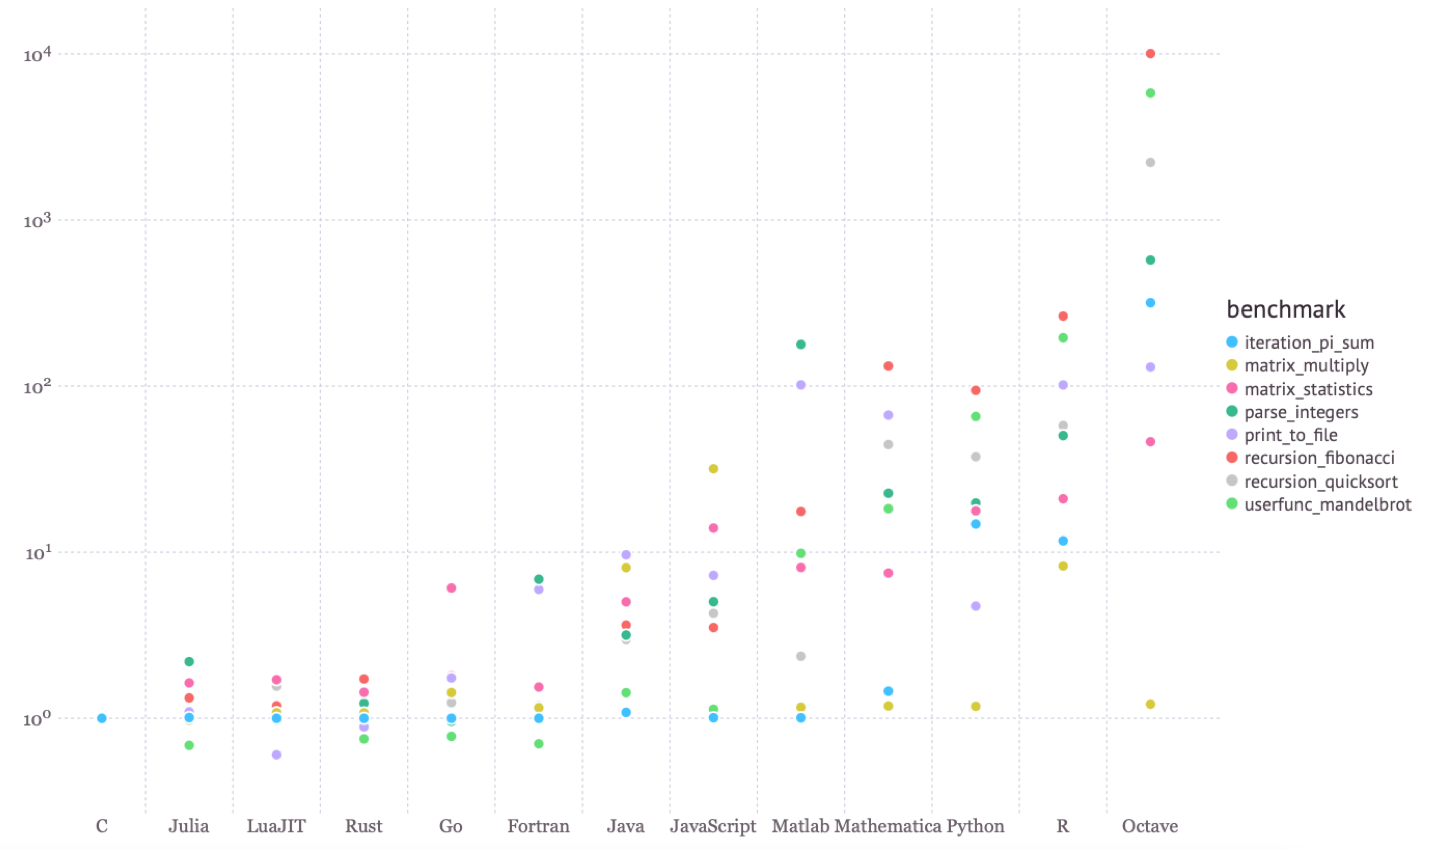
\includegraphics[width=0.8\textwidth]{figures/chapter-2/julia.png}
    \caption{Julia benchmarks from \href{https://julialang.org/benchmarks/}{Julia website}}
    \label{fig:julia}
\end{figure}






%%%%%%%%%%%%%%%%%%%%%%%%%%%%%%%%%%%%%%%%%%%%%%%%%%%
%                  2. Table
%%%%%%%%%%%%%%%%%%%%%%%%%%%%%%%%%%%%%%%%%%%%%%%%%%%
\section{Table}

Here are a table example.

\begin{table}[h]
    \centering
    \caption{Ambient noise package}
    \label{tab:noise-package}
    %\begin{tabular}{c|cccp{6em}p{3em}c}
    \begin{tabular}{m{2cm}<{\centering}m{2cm}<{\centering}m{2.5cm}<{\centering}m{2.5cm}<{\centering}m{1cm}<{\centering}}
        \toprule
        Package   & Language & Multiprocessing & Multithreading & GPU   \\

        \midrule
        SeisNoise.jl &  Julia & \checkmark  & \checkmark & \checkmark \\
        NoisePy & Python & \checkmark & & \checkmark \\
        Mirmex &  C++ & &  \checkmark & \checkmark \\
        CC-FJ  & Python with C++ & & \checkmark  & \\
        NoiseCorr & MATLAB & \checkmark & & \\
        \bottomrule
    \end{tabular}

\end{table}





%%%%%%%%%%%%%%%%%%%%%%%%%%%%%%%%%%%%%%%%%%%%%%%%%%%
%                  3. algorithm
%%%%%%%%%%%%%%%%%%%%%%%%%%%%%%%%%%%%%%%%%%%%%%%%%%%

\section{Algorithm}

Here are an algorithm example.

\begin{algorithm}[h]
    \SetAlgoLined
  
    Choose initial $m_0$,$S(m_0)$\;
    Compute $\pi_{post}(m|d_{obs})$\;
    \For{$k = 0,\dots,N-1$}{
        \eIf{$k<N_k$}{
            Define $S(m)=S_{time}(m)$\;
        }{
            \If{$k<N_k+M_{mag}$}{
                Estimate $M_0$ with formula XX\;
        }
        Define $S(m)=S_{time}(m)$\;
        }
        Draw sample $y$ with random walk with formula 17\;
        Compute $\pi_{post}(y|d_{obs})$\;
        Compute $\beta(m_k,m_{k+1}) = min \biggl\{ \frac{\pi_{post}(m_{k+1}|d_{obs})} {\pi_{post}(m_{k}|d_{obs})}, 1   \biggr\}$ \;
        Draw random number $u \sim u([0,1])$\;
        \eIf{$u<\beta(m_k,m_{k+1})$}{
            Accept: set $m_{k+1}=y$\;
        }{
            Reject: set $m_{k+1}=m_k$\;
        }
    }
    \caption{MCMTpy algorithm to sample proposal distribution $\pi_{post}(m|d_{obs})$}
    \label{algo:MCMTpy}
\end{algorithm}






%%%%%%%%%%%%%%%%%%%%%%%%%%%%%%%%%%%%%%%%%%%%%%%%%%%
%                  4. Code
%%%%%%%%%%%%%%%%%%%%%%%%%%%%%%%%%%%%%%%%%%%%%%%%%%%

\section{Code}


%%%% directly %%%%
% Insert Python code showing below.

% \begin{pythoncode}
% import numpy as np
% """
%     Annotation here.
% """
% # Annotation here.
% def main():
%     for i in range(0,10,1):
%         if i == 1:
%             print("Hello world")

% # Annotation here.
% if __name__ == "__main__":
%     main()
% \end{pythoncode}


%%%% from file %%%%
Insert Python code from files.





\clearpage